\label{sec:model-usecase}
In this section we describe, with our model, the information disclosure and migration alteration attacks detailed in Section~\ref{sec:model-attacks}.
We prove the feasibility of detecting security violations with each attack, using the migration algorithms presented in Section~\ref{sec:migration}.
We describe a virtual topology and verify that the initial setup is respecting the security properties previously defined.
We limit the description of the different axioms used by SNARK for simplicity of reading.
The full implementation of the use case in SNARK is described in Appendix~\ref{appendix:snark-code}.

We have implemented a simulator to generate the formal trace of the migration.
This work includes the topology, the algorithm used, the attacks on the migration process and the different rights users have on the infrastructure.

\subsubsection{Use case setup}
We have set up a network topology with six nodes, as depicted in Figure~\ref{fig:usecase-topo}

\begin{figure*}[htbp]



\tikzset{every picture/.style={line width=0.75pt}} %set default line width to 0.75pt        

\begin{tikzpicture}[x=0.75pt,y=0.75pt,yscale=-1,xscale=1]
%uncomment if require: \path (0,787.8333282470703); %set diagram left start at 0, and has height of 787.8333282470703

%Straight Lines [id:da7362912874212684] 
\draw [line width=1.5]    (217,249.33) -- (494,256) ;


%Straight Lines [id:da12239289508861262] 
\draw [line width=1.5]    (100,320) -- (217,249.33) ;


%Straight Lines [id:da40069379617810275] 
\draw [line width=1.5]    (226,398) -- (351,327) ;


%Straight Lines [id:da7000477419707168] 
\draw [line width=1.5]    (100,320) -- (226,398) ;


%Straight Lines [id:da4669112798901247] 
\draw [line width=1.5]    (230,405.33) -- (507,412) ;


%Straight Lines [id:da8512152422950844] 
\draw [line width=1.5]    (517,408) -- (510,260.33) ;


%Straight Lines [id:da12510362571528755] 
\draw [line width=1.5]    (514,413) -- (361,328.33) ;


%Straight Lines [id:da33197427034782157] 
\draw [line width=1.5]    (504,257) -- (369,328) ;


%Straight Lines [id:da19303419211846296] 
\draw [line width=1.5]    (363,321) -- (232,257) ;


%Image [id:dp07311130989675296] 
\draw (97.5,329) node  {
\includegraphics[width=52.5pt,height=52.5pt]{figures/router-158644_1280.png}};
%Image [id:dp12239452759411629] 
\draw (507.5,258.5) node  {
\includegraphics[width=52.5pt,height=52.5pt]{figures/router-158644_1280.png}};
%Image [id:dp678906579337467] 
\draw (218.5,413.75) node  {
\includegraphics[width=52.5pt,height=52.5pt]{figures/router-158644_1280.png}};
%Image [id:dp34355805397684036] 
\draw (507.5,413.75) node  {
\includegraphics[width=52.5pt,height=52.5pt]{figures/router-158644_1280.png}};
%Image [id:dp32408575207048074] 
\draw (360.5,329) node  {
\includegraphics[width=52.5pt,height=52.5pt]{figures/router-158644_1280.png}};
%Image [id:dp8786300863621592] 
\draw (218.5,258.5) node  {
\includegraphics[width=52.5pt,height=52.5pt]{figures/router-158644_1280.png}};


% Text Node
\draw (221,268) node  [align=left] {A};
% Text Node
\draw (102,338) node  [align=left] {B};
% Text Node
\draw (223,424) node  [align=left] {E};
% Text Node
\draw (364,340) node  [align=left] {C};
% Text Node
\draw (512,271) node  [align=left] {D};
% Text Node
\draw (514,424) node  [align=left] {F};


\end{tikzpicture}

\caption{Network topology of the use case.}
\label{fig:usecase-topo}

\end{figure*}


In addition to the topology, we name the time points of the different steps during the migration process based on the number of iterations (see Figure~\ref{fig:time-points}).
We define the first two basic time points time-0 and time-1 to respectively represent the initial situation and the beginning of the migration process. The last time point varies, depending on the length of execution of the migration.


\begin{figure}[htbp]
\centering
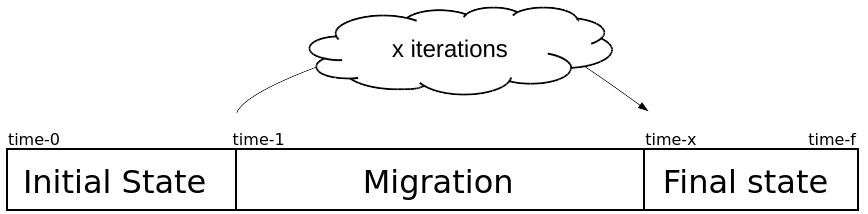
\includegraphics[scale=0.5]{figures/time-points-evolution} 
\caption{Time points of the migration process.\label{fig:time-points}}
\end{figure}

\subsubsection{Initial Situation}
In this section, we consider the network topology prior to any migration.
We solely have the axioms related to the virtual topology, the corresponding users, and the data carried across the network.
We formulate our question to SNARK and verify that the confidentiality is already established prior to the migration (question and answer in Listing~\ref{lst:init-conf-q} and~\ref{lst:init-conf-a}, respectively).

\lstset{numbers=left,numberstyle=\tiny,numbersep=5pt,language=Lisp,
  stringstyle=\ttfamily\small,basicstyle=\ttfamily\footnotesize,
  showstringspaces=false,breaklines=true,keywordstyle=\color{black},}

\begin{lstlisting}[caption=SNARK question to validate the initial situation., label=lst:init-conf-q] 
(find-all '(ans ?d.data ?t.time-interval)
 '(and
 (data-confidentiality ?d.data ?t.time-interval)
(non-empty ?t.time-interval))
 :name 'data-confidentiality-preservation-conjecture
 :num-answers 1
 :time-limit 30  
 :print-derived :print)

;;; search for a data-confidentiality breach:
;;; find all data for which data-confidentiality
;;; has been maintained


(find-all '(ans ?n.node ?t.time-interval)
 '(and
 (node-confidentiality ?n.node ?t.time-interval)
(non-empty ?t.time-interval))
 :name 'node-confidentiality-preservation-conjecture
 :num-answers 1
 :time-limit 30  
 :print-derived :print)

;;; search for a node-confidentiality breach:
;;; find all nodes for which node-confidentiality 
;;; has been maintained
\end{lstlisting}

%\GB{could you comment a bit about what piece of SNARK response  in Lst.~\ref{lst:init-conf-a} gives away the result?}
The interpretation of results provided by SNARK depends on how the question has been formulated.
Lines 1 and 15 from Listing~\ref{lst:init-conf-q} contain requests for the format of the answer.
In these lines, we request SNARK to verify if both nodes and data have their confidentiality respected. The answer will display the time intervals verifying the preservation.
Lines 5 and 15 of Listing~\ref{lst:init-conf-a} hold the answer.
We can establish from line 5 that data-1 has its confidentiality respected (and it is the only one used in our experiment).
At line 15, we have proven that node-1 is not compromised.
The same goes for all the other nodes of the topology, 
for the sake of brevity, these proofs have been omitted.
%but we do not provide the print out in this paper.

\begin{lstlisting}[caption=SNARK validating the initial situation, label=lst:init-conf-a] 
(Row 69
(OR ($$TIME-PP-NOT-BEFORE TIME-0 TIME-1) 
(= (SOME-USER1 DATA-1 (MAKE-INTERVAL TIME-0 TIME-1)) USER-2))
(RESOLVE 66 NON-EMPTY-IF-TIME-POINTS-ORDERED)
Answer (ANS (ANS DATA-1 (MAKE-INTERVAL TIME-0 TIME-1)))) 

(OR ($$TIME-PP-NOT-BEFORE TIME-0 TIME-1)
 (= (SOME-USER1 (SOME-DATA NODE-A (MAKE-INTERVAL TIME-0 TIME-1)) (MAKE-INTERVAL TIME-0 TIME-1)) USER-2)
 (= (SOME-USER NODE-A (MAKE-INTERVAL TIME-0 TIME-1)) USER-2)
 (NOT (DATA-AT-NODE (SOME-DATA NODE-A (MAKE-INTERVAL TIME-0 TIME-1)) NODE-A (MAKE-INTERVAL TIME-0 TIME-1)))
 (NOT
  (DATA-ISAUTHORIZED USER-1 (SOME-DATA NODE-A (MAKE-INTERVAL TIME-0 TIME-1))
   (MAKE-INTERVAL TIME-0 TIME-1))))
   (RESOLVE 115 NON-EMPTY-IF-TIME-POINTS-ORDERED)
   Answer (ANS (ANS NODE-A (MAKE-INTERVAL TIME-0 TIME-1)))) 
\end{lstlisting}


\subsubsection{Information Disclosure attack}
%\GB{are both attacks directed against both migration algorithms}
%\FC{No, but I forgot to mention that we assign an attack per algorithm}
This attack considers two users, one legitimate and one attacker.
The attacker is a collocated user.
In this scenario, the iterative migration algorithm will be used.
During the initial phase, only the legitimate user is active.
The migration process starts and nodes and links are being migrated, one after another.
At some point during the migration, the attacker will start his attack to gain access to the data carried through the VN.
This results into the generation of two predicates, one about the attacker reading the data, and the other about him not being authorized to do so. 
When the migration process ends, the data has been compromised.
In SNARK, the data has been named data-1 and the migration ends at time point time-9.
We formulate our question to SNARK at line 1 from Listing~\ref{lst:not-data-conf-q}.

% \begin{figure}[h]
% \centering
% \includegraphics[scale=0.5]{not-data-confidentiality-question}
% \caption{SNARK question to detect the data confidentiality violation.\label{fig:not-data-conf-q}}
% \end{figure}
% \begin{figure}[h]
% \centering
% \includegraphics[scale=0.5]{not-data-confidentiality-answer}
% \caption{SNARK detecting the data confidentiality violation\label{fig:not-data-conf-a}}
% \end{figure}
\begin{lstlisting}[caption=SNARK question to detect the data confidentiality violation., label=lst:not-data-conf-q] 
   (find-all '(ans ?d.data ?t.time-interval)
             '(and
       (not(data-confidentiality ?d.data ?t.time-interval))
         (non-empty ?t.time-interval))
         :name 'data-conf-preservation-conjecture
         :num-answers 1
         :time-limit 30
         :print-derived :print)
;;; search for a data-confidentiality breach:
;;; find all data for which data-confidentiality has been maintained

\end{lstlisting}
\begin{lstlisting}[caption=SNARK detecting the data confidentiality violation., label=lst:not-data-conf-a] 
(Row 2112  
(OR
 (NOT
  (= (MAKE-INTERVAL TIME-0 ?X.TIME-POINT)
   (MAKE-INTERVAL (MAX-TIME ?Y.TIME-POINT ?Z.TIME-POINT) (MIN-TIME ?U.TIME-POINT ?V.TIME-POINT))))
 (NOT (SETLINK0 NODE-B ?W.NODE (MAKE-INTERVAL ?Y.TIME-POINT ?U.TIME-POINT)))
 (NOT (SETLINK ?W.NODE NODE-A (MAKE-INTERVAL ?Z.TIME-POINT ?V.TIME-POINT)))
 ($$TIME-PP-NOT-BEFORE TIME-9 (MIN-TIME TIME-1 ?X.TIME-POINT)) ($$TIME-PP-NOT-BEFORE TIME-4 TIME-9)
 (NOT (= (MAKE-INTERVAL TIME-4 TIME-9) (MAKE-INTERVAL TIME-0 TIME-9))) ($$TIME-PP-NOT-BEFORE TIME-4 TIME-9)
 (DATA-ISAUTHORIZED ATTACKER DATA-1 (MAKE-INTERVAL TIME-4 TIME-9)))
   (RESOLVE 1938 18)
   Answer (ANS (ANS DATA-1 (MAKE-INTERVAL TIME-4 TIME-9)))) 
\end{lstlisting}
We can see that SNARK confirms the data confidentiality violation at line 12 from Listing~\ref{lst:not-data-conf-a}.
Since the attack started during the migration (i.e after time point time-1), SNARK detects the beginning of the confidentiality violation at time point time-4.
Line 10 highlights that the attacker does not have the authorization to read the data.
%\GB{could you point out directly which line you are referring to by labeling and referring to independent lines in the listing?}

\subsubsection{Migration alteration attack}
Exploiting the physical nodes leverages other aspects of the security the infrastructure.
The initial situation is similar to the previous scenario but we use the move-based migration algorithm instead.
The attacker is located in the network infrastructure.
The attacker can render physical nodes unavailable to trigger the migration process and will intercept and modify the configuration data sent by the hypervisor. 
Therefore, we have two new predicates appearing during the migration, the fact that A accesses a node, and the fact that A is not authorized to do so.
%\GB{should this fact be generated. Should this be rather the absence of an is\_authorized predicate that would indicate the attack?}
%\FC{Answered by email}
At line 1 in Listing~\ref{lst:not-node-conf-q}, we ask SNARK to find all the nodes in which there is a confidentiality breach.

\begin{lstlisting}[caption=SNARK question to detect the node confidentiality violation., label=lst:not-node-conf-q] 
   (find-all '(ans ?n.node ?t.time-interval)
             '(and
       (not(node-confidentiality ?n.node ?t.time-interval))
               (non-empty ?t.time-interval))
             :name 'node-conf-violation-conjecture
             :num-answers 1
             :time-limit 30
             :print-derived :print)

   ;;; search for a node-confidentiality breach:
   ;;; find all nodes for which node-confidentiality has not been maintained
\end{lstlisting}
The node confidentiality breach is then proven by SNARK for node-a at line 5 in Listing~\ref{lst:not-node-conf-a}.
Similarly to the previous information disclosure scenario, the attack starts after the beginning of the migration process but before it ends.
SNARK finds the beginning of the attack on node-a starting at time point time-1.
In addition to that, Line 1 explains that the confidentiality of the node is broken by user 2 (i.e. the attacker).
%\GB{again, please provide line numbers for the reviewer to ``see something''}

\begin{lstlisting}[caption=SNARK detecting the node confidentiality violation., label=lst:not-node-conf-a] 
(OR (NODE-ISAUTHORIZED USER-2 NEW_NODE-A (MAKE-INTERVAL TIME-1 ?X.TIME-POINT))
 ($$TIME-PP-NOT-AFTER ?X.TIME-POINT TIME-3))
   (REWRITE (RESOLVE 585 819) :CODE-FOR-$$TIME-PP-INTERSECTION)
   Answer (ANS (ANS NEW_NODE-A (MAKE-INTERVAL TIME-1 TIME-3)))) 
\end{lstlisting}

The proof related to the other predicates (availability, integrity, and configuration confidentiality) is identical in essence, thus we do not include it here.